% Part I > Certificates. Step 5 of the integrity argument (AUDIT.md s2):
% machine-checked certificates are the check that scales and ignores
% provenance; they got cheap; they catch what review missed; and verifiers are
% where AI improves. Then "necessary, not sufficient": the paper/code slide,
% reframed as auditability, and the three layers as the hand-off to Part II.
\section{Certificates}

% [2 min] Introduces AI-assisted formalization as a concept: the pipeline
% (human statement and blueprint -> AI formalizes and proves -> kernel checks
% -> registered certificate), then what it addresses from the community-response
% section and what it leaves open. Replaces the earlier problem/certificate
% table (same content, Kyle asked for a non-table slide).
\begin{frame}{AI-assisted formalization}
  \centering
  \begin{tikzpicture}[x=1cm, y=1cm, font=\sffamily\footnotesize]
    \useasboundingbox (0,0.1) rectangle (14.3,-5.9);
    % ---- definition --------------------------------------------------------
    \node[anchor=north west, text width=14.2cm, align=flush left, inner sep=0pt, font=\sffamily\small]
      at (0,0.05)
      {AI translates mathematics into a proof assistant such as Lean and fills in the proofs.
       A small trusted kernel checks every step. Humans write, or review, what is being proved.};
    % ---- pipeline ----------------------------------------------------------
    \node[stage=PennBlue, minimum width=2.9cm, minimum height=1.05cm] (p1) at (1.65,-1.5)
      {Statement \& blueprint\\[-1pt]{\scriptsize\color{black!60}human}};
    \node[stage=tlPurple, minimum width=2.9cm, minimum height=1.05cm] (p2) at (5.35,-1.5)
      {Formalize \& prove\\[-1pt]{\scriptsize\color{black!60}AI agents}};
    \node[stage=PennGreen, minimum width=2.9cm, minimum height=1.05cm] (p3) at (9.05,-1.5)
      {Kernel check\\[-1pt]{\scriptsize\color{black!60}Lean}};
    \node[stage=PennGold, minimum width=2.9cm, minimum height=1.05cm] (p4) at (12.75,-1.5)
      {Certificate\\[-1pt]{\scriptsize\color{black!60}registry, e.g.\ Palomar}};
    \foreach \u/\v in {p1/p2, p2/p3, p3/p4} \draw[flow] (\u) -- (\v);
    \draw[flow=PennBlue, dashed] (p3.south) .. controls +(0,-0.55) and +(0,-0.55) .. (p1.south);
    \node[note, fill=white, inner sep=1pt] at (5.35,-2.48) {a human checks that the formal statement matches the paper};
    % ---- what it addresses / what stays open --------------------------------
    \node[anchor=north west, inner sep=0pt, font=\sffamily\small\bfseries, text=PennGreen] at (0,-2.95)
      {What it addresses};
    \node[anchor=north west, inner sep=0pt, font=\sffamily\small\bfseries, text=PennRed] at (7.35,-2.95)
      {What stays open};
    \node[anchor=north west, text width=6.85cm, align=flush left, inner sep=0pt, font=\sffamily\scriptsize] at (0,-3.4) {%
      \begin{itemize}\setlength{\itemsep}{1pt}
        \item \textbf{Review capacity.} Referees review a page of statements, not 60 pages of proof.
        \item \textbf{Undisclosed AI.} The check does not depend on who, or what, wrote the proof.
        \item \textbf{Bypassed review.} Verify and register a result before announcing it.
        \item \textbf{Credit.} Registries record what produced each result.
      \end{itemize}};
    \node[anchor=north west, text width=6.85cm, align=flush left, inner sep=0pt, font=\sffamily\scriptsize] at (7.35,-3.4) {%
      \begin{itemize}\setlength{\itemsep}{1pt}
        \item \textbf{Statement fidelity.} Compiling is not saying the same thing (Navier--Stokes).
        \item \textbf{Understanding.} Millions of machine-written lines explain nothing.
        \item \textbf{Significance and ideas.} Neither is a formal property.
        \item \textbf{Access and coverage.} Frontier compute; thin libraries in PDE and applied probability.
      \end{itemize}};
  \end{tikzpicture}
  \slidesources{Tao, \emph{Palomar}, blog, 18 Aug 2026 \textbullet{} Bastounis, Circelli \& Hansen, arXiv 2610.08144 \textbullet{} research notes 01--03}
\end{frame}

% [1 min] The cost of formalization collapsed: each row pairs a human-era
% effort with an AI-era one on a comparable target. Log scale in days,
% x = 1.9cm * log10(days). Human: Strong PNT 18 months (Tao--Kontorovich);
% FLT 5-year EPSRC grant from 2024 (unfinished when the agents finished);
% Odd Order theorem alone, 6 years (ITP 2013). AI: Strong PNT 3 weeks (Math,
% Inc.); FLT 11 days (Anthropic); CFSG 24 days (Axiom). AI figures are
% self-reported (research/01 s1); CFSG has no independent build yet.
\begin{frame}{Formalization got cheap}
  \centering
  \begin{tikzpicture}[x=1cm, y=1cm, font=\sffamily\scriptsize,
      hbar/.style={fill=black!28, draw=none},
      abar/.style={fill=PennBlue, draw=none},
      blabel/.style={anchor=west, inner sep=0pt, text=black!75},
      rowlab/.style={anchor=north west, text width=3.9cm, align=flush left, inner sep=0pt, font=\sffamily\footnotesize}]
    \useasboundingbox (0,0.2) rectangle (14.3,-5.9);
    \def\xo{4.3}
    % legend
    \fill[hbar] (\xo,0.0) rectangle ++(0.35,-0.2);
    \node[blabel] at (\xo+0.45,-0.1) {human-led};
    \fill[abar] (\xo+2.2,0.0) rectangle ++(0.35,-0.2);
    \node[blabel] at (\xo+2.65,-0.1) {AI agents (self-reported)};
    % rows: \row{y}{label}{human cm}{human text}{AI cm}{AI text}
    \foreach \y/\lab/\h/\htext/\a/\atext in {
        -0.55/{\textbf{Strong Prime Number Theorem}}/5.20/{18 months: Tao--Kontorovich}/2.51/{3 weeks: Gauss (Math, Inc.), 2025},
        -2.15/{\textbf{Fermat's Last Theorem}\\{\scriptsize\color{black!60}agents built on Buzzard's project}}/6.20/{5-year grant from 2024, unfinished}/1.98/{11 days: Claude agents, Sep 2026},
        -3.75/{\textbf{Finite simple groups}\\{\scriptsize\color{black!60}human: Odd Order theorem alone}}/6.35/{6 years: Odd Order in Coq (2012)}/2.62/{24 days: the whole classification (Axiom), Oct 2026}} {
      \node[rowlab] at (0,\y+0.05) {\lab};
      \fill[hbar] (\xo,\y) rectangle (\xo+\h,\y-0.42);
      \node[blabel] at (\xo+\h+0.12,\y-0.21) {\htext};
      \fill[abar] (\xo,\y-0.52) rectangle (\xo+\a,\y-0.94);
      \node[blabel] at (\xo+\a+0.12,\y-0.73) {\atext};
    }
    % log axis in days
    \draw[black!40, line width=0.5pt] (\xo,-4.95) -- (\xo+6.6,-4.95);
    \foreach \v/\t in {0/1 day, 1.61/1 week, 2.81/1 month, 4.87/1 year, 6.20/5 years} {
      \draw[black!40] (\xo+\v,-4.95) -- (\xo+\v,-5.05);
      \node[note, anchor=north] at (\xo+\v,-5.08) {\t};
      \draw[black!8, line width=0.4pt] (\xo+\v,-4.95) -- (\xo+\v,-0.4);
    }
    \node[note, anchor=north west, text width=9.5cm] at (\xo,-5.45)
      {Log scale. The AI-era figures come from the companies; the finite-simple-groups build has not been independently reproduced.};
  \end{tikzpicture}
  \slidesources{Math, Inc., Strong PNT (2025) \textbullet{} Anthropic, FLT (Sep 2026) \textbullet{} Axiom, CFSG (Oct 2026) \textbullet{} Gonthier et al., ITP 2013 \textbullet{} research note 01, \S1}
\end{frame}

% [1.5 min] Certificates catch what review missed. Column 1 is independent
% (community audit; withdrawals all outside Lean coverage, research/01 s5).
% Columns 2-3 are Axiom's own reports (research/01 s2-3).
\begin{frame}{Certificates catch what review missed}
  \centering
  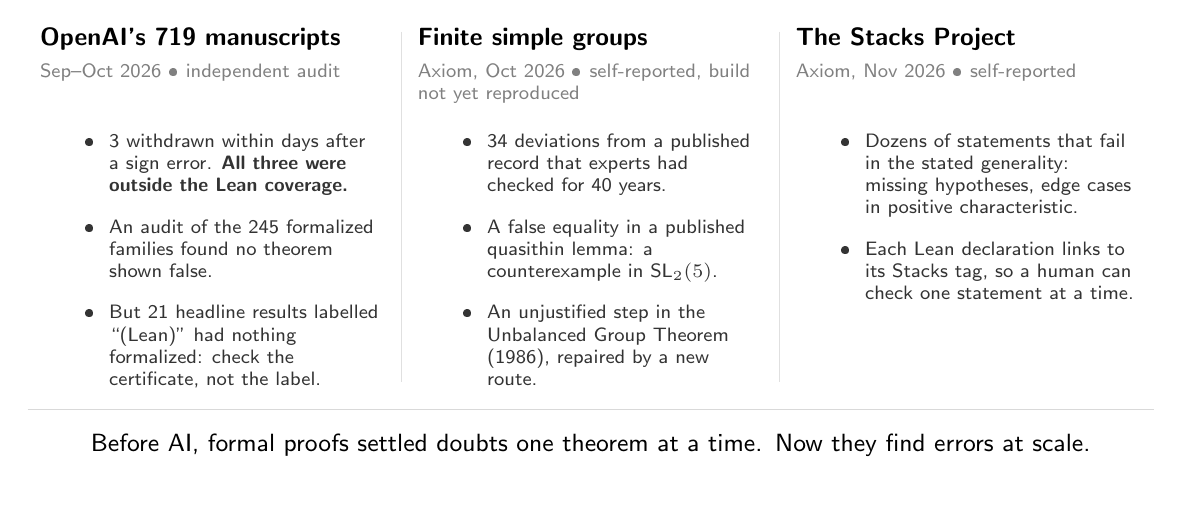
\begin{tikzpicture}[x=1cm, y=1cm,
      chead/.style={anchor=north west, text width=4.3cm, align=flush left, inner sep=0pt,
                    font=\sffamily\small\bfseries},
      ctag/.style={anchor=north west, text width=4.3cm, align=flush left, inner sep=0pt,
                   font=\sffamily\scriptsize, text=black!50},
      cbody/.style={anchor=north west, text width=4.3cm, align=flush left, inner sep=0pt,
                    font=\sffamily\scriptsize, text=black!80}]
    \useasboundingbox (0,0) rectangle (14.3,-5.9);
    \foreach \x in {4.75, 9.55} \draw[black!12, line width=0.5pt] (\x,-0.05) -- (\x,-4.5);
    % column 1
    \node[chead] at (0.15,0) {OpenAI's 719 manuscripts};
    \node[ctag] at (0.15,-0.45) {Sep--Oct 2026 \textbullet{} independent audit};
    \node[cbody] at (0.15,-0.95) {%
      \begin{itemize}\setlength{\itemsep}{3pt}
        \item 3 withdrawn within days after a sign error. \textbf{All three were outside the Lean coverage.}
        \item An audit of the 245 formalized families found no theorem shown false.
        \item But 21 headline results labelled ``(Lean)'' had nothing formalized: check the certificate, not the label.
      \end{itemize}};
    % column 2
    \node[chead] at (4.95,0) {Finite simple groups};
    \node[ctag] at (4.95,-0.45) {Axiom, Oct 2026 \textbullet{} self-reported, build not yet reproduced};
    \node[cbody] at (4.95,-0.95) {%
      \begin{itemize}\setlength{\itemsep}{3pt}
        \item 34 deviations from a published record that experts had checked for 40 years.
        \item A false equality in a published quasithin lemma: a counterexample in SL$_2(5)$.
        \item An unjustified step in the Unbalanced Group Theorem (1986), repaired by a new route.
      \end{itemize}};
    % column 3
    \node[chead] at (9.75,0) {The Stacks Project};
    \node[ctag] at (9.75,-0.45) {Axiom, Nov 2026 \textbullet{} self-reported};
    \node[cbody] at (9.75,-0.95) {%
      \begin{itemize}\setlength{\itemsep}{3pt}
        \item Dozens of statements that fail in the stated generality: missing hypotheses, edge cases in positive characteristic.
        \item Each Lean declaration links to its Stacks tag, so a human can check one statement at a time.
      \end{itemize}};
    % conclusion
    \draw[black!15, line width=0.4pt] (0,-4.85) -- (14.3,-4.85);
    \node[anchor=north, text width=13.5cm, align=center, inner sep=0pt, font=\sffamily\small]
      at (7.15,-5.15)
      {Before AI, formal proofs settled doubts one theorem at a time. Now they find errors at scale.};
  \end{tikzpicture}
  \slidesources{borism/openai-math-slop, issue \#2 \textbullet{} OpenAI release record (Wikipedia) \textbullet{} Axiom, CFSG (Oct 2026) and Stacks (Nov 2026) \textbullet{} research note 01, \S\S2--3, 5}
\end{frame}

% [1.5 min] No verifier, no flywheel (AcadMathSci A.5; the report's view, not
% a measurement). For this audience: AI improves fastest where outputs can be
% checked automatically, because the check is a reward signal. AlphaProof
% figures from A.5. The Yue et al. mechanism (RLVR sharpens rather than
% extends) is still on the verify list, so it is not on the slide.
\begin{frame}{No verifier, no flywheel}
  \centering
  \begin{tikzpicture}[x=1cm, y=1cm, font=\sffamily\footnotesize]
    \useasboundingbox (0,0) rectangle (14.3,-5.9);
    % ---- the loop -----------------------------------------------------------
    \node[stage=tlPurple, minimum width=2.6cm] (m) at (1.75,-1.1) {Model\\[-1pt]{\scriptsize\color{black!60}proposes a proof}};
    \node[stage=black, minimum width=2.6cm] (f) at (5.35,-1.1) {Formal proof\\[-1pt]{\scriptsize\color{black!60}attempt}};
    \node[stage=PennGreen, minimum width=2.6cm] (k) at (3.55,-3.15) {Kernel check\\[-1pt]{\scriptsize\color{black!60}pass or fail}};
    \draw[flow] (m) -- (f);
    \draw[flow] (f) -- (k);
    \draw[flow=PennGreen] (k) -- node[note, left=3pt, align=right] {reward:\\training signal} (m);
    \node[note, anchor=north, text width=6.2cm, align=center] at (3.55,-4.0)
      {AlphaProof autoformalized about 1M problems into about 80M Lean statements to train on this loop.};
    % ---- the argument -------------------------------------------------------
    \node[anchor=north west, text width=6.6cm, align=flush left, inner sep=0pt, font=\sffamily\small] at (7.6,-0.2) {%
      \begin{itemize}\setlength{\itemsep}{5pt}
        \item Where a result can be checked automatically, every attempt is a training signal. AcadMathSci: Lean is becoming the way AI checks its own work.
        \item Where it can't (modelling choices, significance, exposition), a person has to judge every output.
        \item So capability ``will stay uneven across the mathematical sciences''.
      \end{itemize}};
    % conclusion
    \draw[black!15, line width=0.4pt] (0,-4.85) -- (14.3,-4.85);
    \node[anchor=north, text width=13.5cm, align=center, inner sep=0pt, font=\sffamily\small]
      at (7.15,-5.15)
      {AI gains arrive first where results can be checked. Formalizing a field puts it on that side.};
  \end{tikzpicture}
  \slidesources{Reisinger et al., AcadMathSci, Oct 2026 (\S1.2; A.5, the report's assessment)}
\end{frame}

% [1 min] Navier--Stokes revisited, reframed in talk-v2 as auditability: the
% drift could be pinned to exact lemmas only because formal code existed.
% Originally: the certificate compiled, and the code
% still says something other than the paper. They do NOT claim the paper is
% wrong; the argument was about credit, not correctness.
\begin{frame}{The paper and the code disagree}
  \small\sffamily
  \begin{columns}[T]
    \begin{column}{0.54\textwidth}
      \textbf{Navier--Stokes} (Bastounis, Circelli \& Hansen, Oct 2026)
      \begin{itemize}\footnotesize
        \item The paper's estimate (8.19) needs $m{+}4$ derivatives; the matching Lean theorem assumes $m{+}5$, and the pattern repeats.
        \item The paper's pressure bound depends on one quantity; the Lean bound depends on two, and is proved by a different route.
        \item They do not claim the paper is wrong.
      \end{itemize}
      \medskip
      \textbf{OpenAI's 719 manuscripts} (community audit of 245 formalized families)
      \begin{itemize}\footnotesize
        \item About 210 consistent at the level of statements; no theorem shown false.
        \item 21 headline results marked ``(Lean)'' were not formalized; 5 formalized only a supporting lemma.
      \end{itemize}
    \end{column}
    \begin{column}{0.42\textwidth}
      \vspace{0.4cm}
      \begin{tikzpicture}
        \node[draw=PennRed!45, fill=PennRed!3, line width=0.6pt, rounded corners=2pt,
              text width=5.3cm, inner sep=0.3cm, align=left, font=\rmfamily\itshape\small] (q)
          {Lean acceptance (compilation) of translation does not imply semantic preservation.};
        \node[anchor=north west, font=\sffamily\scriptsize, text=black!60, inner sep=0pt]
          at ([yshift=-0.15cm]q.south west) {--- Bastounis, Circelli \& Hansen, arXiv 2610.08144};
      \end{tikzpicture}
      \vspace{0.5cm}

      {\footnotesize The drift was found because there was formal code to hold the paper against.\par\smallskip
       A certificate proves \emph{a} theorem. Whether it is \emph{the} theorem is a human question.}
    \end{column}
  \end{columns}
  \slidesources{Bastounis, Circelli \& Hansen, arXiv 2610.08144 \textbullet{} borism/openai-math-slop, issue \#2 \textbullet{} research note 01, \S5}
\end{frame}

% [2 min] The three layers: posed here, answered in Part II.
\begin{frame}{Three layers of checking}
  \centering
  \begin{tikzpicture}[x=1cm, y=1cm]
    \useasboundingbox (0,0.1) rectangle (14.2,-6.0);
    \node[layer=PennGreen, anchor=north west] (k) at (3.6,0)
      {\textbf{Does Lean accept the proof?} Cheap and mechanical. Watch for \texttt{sorry}, extra axioms and kernel bugs.\hfill{\stdone}};
    \node[lbl=PennGreen] at (3.35,-0.72) {1. Kernel};
    \node[layer=PennGold, anchor=north west] (s) at (3.6,-1.8)
      {\textbf{Does the formal statement say what the paper claims?} Scarce: ``will never be solved purely in software'' (Kontorovich). Navier--Stokes drifted here.\hfill{\stopen}};
    \node[lbl=PennGold!85!black] at (3.35,-2.52) {2. Statement};
    \node[layer=PennRed, anchor=north west] (u) at (3.6,-3.6)
      {\textbf{Does anyone understand the proof, and does it match the written one?} Scarce. Machine proofs run to millions of lines.\hfill{\stopen}};
    \node[lbl=PennRed] at (3.35,-4.32) {3. Understanding};
    \node[anchor=north, font=\sffamily\small, text width=12cm, align=center] at (7.8,-5.4)
      {Layer 1 makes correctness cheap and auditable. Layers 2 and 3 stay human: Part II.};
  \end{tikzpicture}
  \slidesources{Research note 01, \S0 \textbullet{} Kontorovich, via AcadMathSci, Oct 2026 (\S2.2) \textbullet{} Bastounis, Circelli \& Hansen, arXiv 2610.08144}
\end{frame}
